\chapter{Modèles de l'apprentissage automatique}\label{chapitre2}
Ce chapitre est consacré aux différents modèles d'apprentissage profonds. Il se focalisera principalement sur les réseaux de neurones convolutifs puisqu'ils ont plus été utilisé dans ce travail que le reste, et il se terminera par un petit détail sur un des modèles renforcé (xgboost) . 
\section{Réseau de neurones artificiels}\label{section12}%\cite{ann1, ann2} 
Le réseau de neurones artificiels est une fonction mathématique s'inspirant du réseau de neurones biologique. Il prend en entrée un vecteur de dimension d qu'il va par la suite transformer en un autre vecteur de dimension k en sortie. Pendant cette transformation, chaque élément de position $i$ du vecteur d'entrée est multiplié par un réel $w_{ij}$ pour donner le vecteur $Sum_j$ de la sortie. L'élément $j$ du vecteur de la sortie est obtenu en faisant la somme des éléments du vecteur $Sum_j$. Pour avoir une forme non linéaire, une fonction non linéaire est appliquée sur la sortie. Les $w_{ij}$ sont appelés les poids de connexions entre les neurones. Chaque vecteur est appelé une couche, ainsi le vecteur d'entrée est appelé la couche d'entrée et celui de sortie la couche de sortie. Une couche intermédiaire est appelée une couche cachée.\\
Soit $I = (I_1, ..., I_d)$ le vecteur d'entrée et $S = (S_1,...,S_k) $ celui de la sortie, $W$ la matrice des poids et $A$ la fonction d'activation. $\forall j = 1..k$ $S_j = A(\sum \limits_{i=1}^d W_{ij}*I_i) $.

L'apprentissage est l'étape de calibrage des paramètres, nous avons quatre modes d'apprentissage: l'apprentissage supervisé, l'apprentissage non supervisé, l'apprentissage semi-supervisé et l'apprentissage par renforcement. Notre travail est basé sur l'apprentissage supervisé.
L'apprentissage supervisé suppose la connaissance au préalable de l'étiquette (valeur à estimer pour une entrée) de chaque individu de l'ensemble de l'échantillon d'entrée.À partir de cet échantillon étiqueté, un algorithme d'apprentissage essaie de trouver une corrélation entre les données et leurs étiquettes en donnant des valeurs aux poids du réseau. Quant à l'apprentissage non supervisé, cette corrélation est obtenue à partir des données non étiquetées.

\subsection{Perception multi-couches (MLP)}
\begin{itemize}
    \item \textbf{Perception} 
\end{itemize}

\begin{figure}[h!]
    \centering
    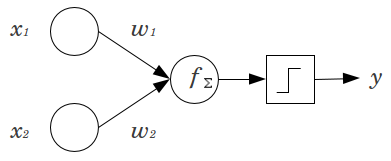
\includegraphics[scale = 0.6]{images/perceptron.png}
    \caption{Perceptron}
    \label{perceptron}
\end{figure}

%\begin{wrapfigure}{r}{5cm}
%\centering
%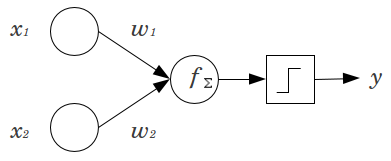
\includegraphics[width = 8cm ]{images/perceptron.png}
%\end{wrapfigure}

Le perception est un réseau de neurone artificiel à une couche d'entrée et une de sortie sans couche cachée. Comme on peut voir un exemple sur la figure \ref{perceptron}, le perception est le modèle de réseau de neurones le plus simple. Son défaut est son incapacité à estimer une fonction non linéaire.\\


\begin{itemize}
    \item \textbf{Perception multi-couches (MLP)}
\end{itemize}


%\begin{wrapfigure}{r}{5cm}
%\centering
%\rule{3cm}{7cm}
%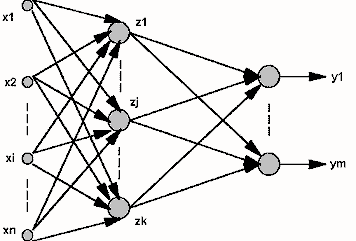
\includegraphics[width = 8cm ]{images/multicouche.png}
%\end{wrapfigure}

Le MLP(Multi-layer perceptron) est un réseau de neurones à au moins une couche cachée. On peut le considérer comme une séquence d'un ensemble de perceptrons. Cette manière de séquencer les perceptrons et d'activer chaque sortie de chaque percetron par une fonction non linéaire émerge un comportement non linéaire permettant ainsi d'estimer les fonctions non linéaire. Le nombre de séquence de perceptron défini la profondeur de l'architecture du réseau. Le MLP augmente le nombre de paramètres(poids) à calibrer, en fonction de l'augmentation de la profondeur. L'augmentation de la profondeur peut facilement amener le modèle à spécialiser le calibrage des poids sur les données d'entrée (sur-apprentissage), ce qui entraîne une mauvaise estimation d'un nouveau exemple.  
\begin{figure}[H]
    \centering
    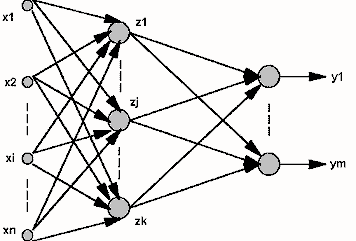
\includegraphics[scale = 0.5]{images/multicouche.png}
    \caption{MLP}
    \label{mlp}
\end{figure}

%\subsection{Réseau de neurones récursifs}
%Le réseau de neurones récursifs est un des modèles de réseau de neurones doté d'une %capacité de mémorisation grâce à son système de récursion et est adapté aux données à %évolution temporelle. Il est très utilisé dans le traitement des langages. Il souffre %énormément de la perte du gradient et de l'explosion de ce dernier. LSTM est un type de %réseau de neurones récursifs permettant de surmonter ce problème.
\subsection{Auto-Encoder}
%\begin{wrapfigure}{r}{4cm}
%\centering
%\rule{3cm}{7cm}
%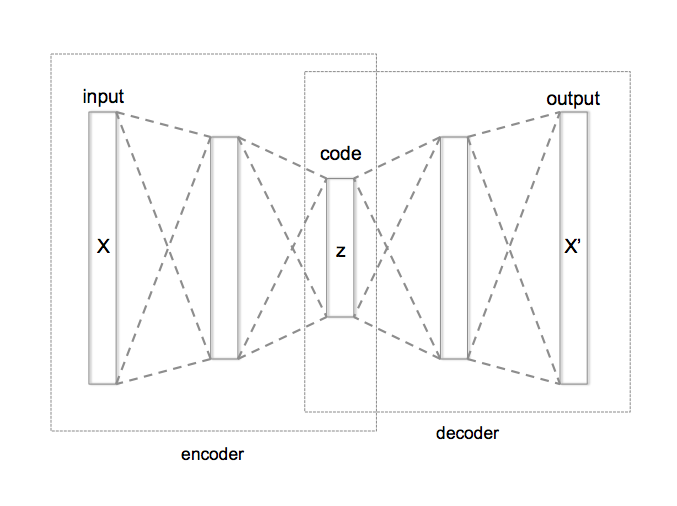
\includegraphics[width = 8cm ]{images/Autoencoder_structure.png}
%\end{wrapfigure}
Un auto-encoder est un réseau de neurones dont sa phase d'apprentissage est non supervisée et chaque sortie du réseau est semblable à l'entrée. Le vecteur résultant est l'une des couches cachée appelée le code qui est un condensé de la représentation de l'entrée, il est comme l'analyse de la composante principale (PCA) mais il permet de plus une représentation non linéaire par rapport au PCA \cite{ann1}. La partie de l'architecture réseau avant l'obtention du code est appelé codeur et celui après le décodeur, comme on le voir sur la figure \ref{autot_encoder}.
\begin{figure}[H]
    \centering
    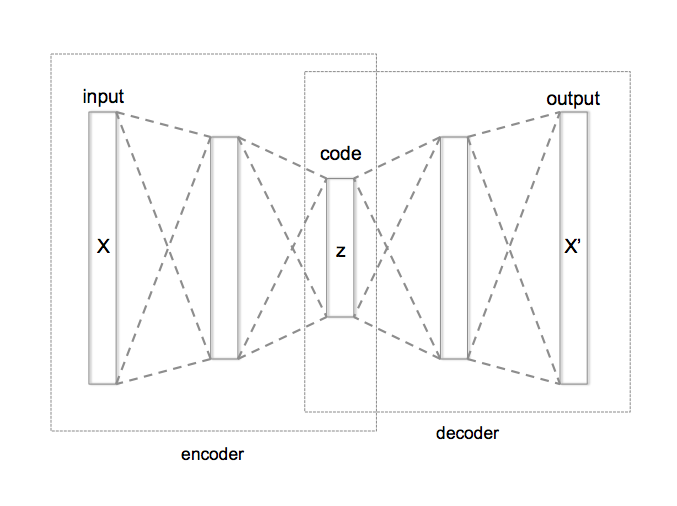
\includegraphics[scale = 0.4]{images/Autoencoder_structure.png}
    \caption{Auto-encoder}
    \label{autot_encoder}
\end{figure}

\section{Réseau de neurones convolutifs (CNN)}
Les réseaux de neurones convolutifs sont de type de réseau de neurone travaillant sur des images en se focalisant sur des caractéristiques locaux de l'image qu'il transforme d'une abstraction à une autre à travers les couches \cite{adavencedCNN}. Il s'inspire du cortex visuel du chat, ce qui le rend plus approprié pour la vision artificielle.\\

Le réseau convolutif permet non seulement l'obtention d'une bonne précision par rapport au réseau de neurone classique mais aussi permet la diminution du nombre de paramètre du réseau à apprendre (les poids) à travers le partage des poids.\\

\textbf{Noyau ou filtre(Kernel), Opération de convolution, Déplacement (strides),  Padding } \\%\cite{}\\
Le noyau est la matrice de paramètres qui se connecte sur la partie locale de l'image pour l'opération de convolution, donc cette partie locale doit avoir la même dimension que le noyau. Le noyau contient alors les paramètres (poids) à apprendre et il sera utilisé pour tout le reste des parties locales de même taille de l'image en faisant passer une fenêtre de déplacement sur l'image. L'opération de convolution est de multiplier case par case les deux matrices pour obtenir une matrice M, puis faire la somme des éléments de M pour l'obtention d'un scalaire qui est le résultat final de la convolution, c'est donc une fonction non inversible. Le déplacement est le nombre de case pour se déplacer vers la droite et en bas pour positionner le noyau sur une nouvelle partie locale de l'image pour une autre opération de convolution. Au coin supérieur gauche de l'image la position du  déplacement est (0,0), puisque une opération complète de convolution donne comme résultat une image intermédiaire A qui est une abstraction de l'ancienne, la valeur de A(i,j) correspond au résultat de l'opération de convolution à la position du déplacement (i,j).À la position (p, q) de déplacement, la prochaine position à droite est (p+1, q) et en bas (p, q+1). On remarque rapidement la diminution de la dimension de l'image , le padding permet d'augmenter la taille de l'image par des zéros pour avoir la même dimension de sortie que l'entrée.\\


\textbf{Fonctionnement}\\
Le réseau convolutif divise la matrice de l'image en des petites matrices(de même taille que le noyau) ordonnées par leurs positions et ces petites matrices passe dans le même réseau de neurones (c'est-à-dire les mêmes poids : noyau) pour donner une nouvelle matrice en sortie qui sera à son tour une entrée d'une nouvelle couche et ainsi de suite jusqu'à la sortie. Dans mon explication ci-dessus certes j'ai fait plus d'abstraction de certains détails, il y a pas que de couches de convolution qui existe, il y à des couches de regroupement (pooling), de couches d'activation (ReLu (généralement utilisé), softMax, tanh, ...), de couche de simplification pour empecher de passer en surapprentissage (dropout, batch normalization, ...) \cite{adavencedCNN}

\begin{figure}[H]
    \centering
    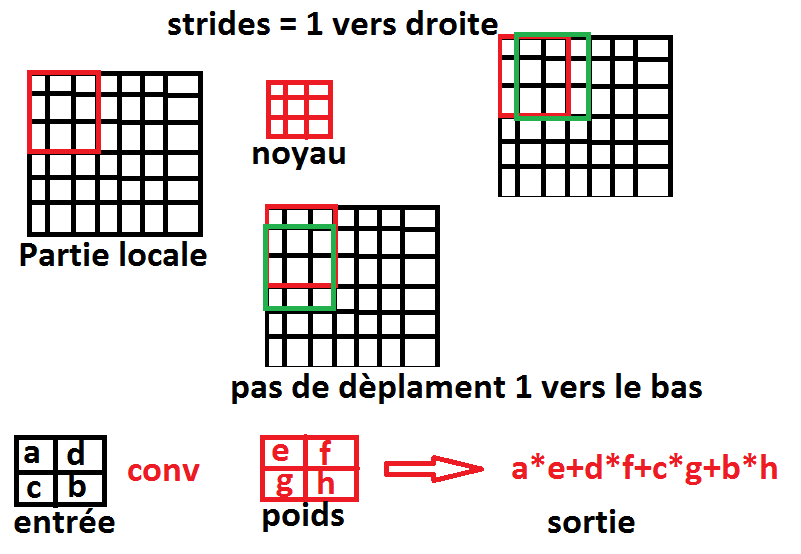
\includegraphics[scale = 0.7]{images/operations_conv.png}
    \caption{fonctionnement du réseau de neurone convolutif}
\end{figure}

\subsection{Couche convolutive}
Plusieurs amélioration de la couche convolutive ont été proposées dans la littérature et ont donné des bons résultats surtout sur la base de données de Image-Net \cite{im1}%plusieurs à cité
Nous avons plusieurs de réseau convolutifs, mais nous avons présenter que quelques en détail.
\begin{figure}[H]
    \centering
    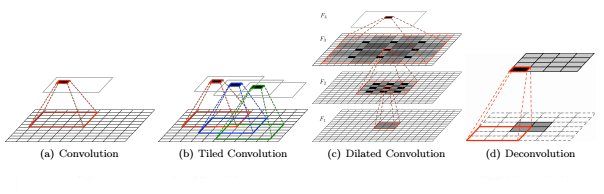
\includegraphics[scale = 0.8]{images/all_cnn.png}
    \caption{Illustration de quelques type de CNN}
\end{figure}
\subsubsection{Tiled convolutional network (TCN)}
Le réseau convolutif d'origine n'utilise qu'un seul noyau qui est partagé entre toutes les parties locales de l'image. Il permet d'éviter des problèmes de translation mais pas d'autres dérangement dans l'image telle la rotation. Le TCN permet d'utiliser à chaque couche convolutive plusieurs noyaux, ainsi permettant plus d'abstractions\cite{tcnn1, tcnn2, tcnn3}. 



\subsubsection{Transposed convolution ou Deconvolution (TC)}
Une couche convolutive de CNN prend une image (matrice) en entrée et retourne une autre image de dimension inférieur ou égale à l'image d'origine, le TC fait l'opération inverse. Le TC transforme chaque case de la matrice de l'image en une petite matrice. Ce n'est pas vraiment une opération inverse du CNN comme l'apparence nous fait croire mais c'est juste le type d'entrées et sorties qui sont inversé. Pour un CNN, les poids se fixent sur une localité et retourne un scalaire tandis pour TC on part d'un scalaire pour arriver à une matrice locale. Pour plus de détail on peut voir \cite{transcd1, transcd2, transcd3,transcd4, transcd5}  
\subsubsection{Dilated convolutional neural}
Le dilated convolution neural élargit de plus le filtre en mettant autant des zéros que nécessaires (un hyper-paramètre à donner) entre une case et ses voisines de la matrice noyau. Pour plus de détail concernant le dilated convolutional le lecteur peut se référer \cite{dilate1, dilate2, dilate3, dilate4}.
\subsubsection{Network in network (NiN)}
Le NiN\cite{nin1} est une des améliorations la plus intéressante par rapport aux précédentes, elle permet dans chaque couche convolutive d'utiliser comme filtre un petit réseau de neurones profonds. C'est-à-dire sur la partie locale, est appliquée un petit réseau de neurones profond au lieu d'un perceptron comme dans le cas du CNN. C'est qui veut dire qu'une couche de NiN est constituée d'une couche de convolution de noyau (k, m) suivi par plusieurs couches de convolution de noyau (1,1) chacune.

\begin{figure}[H]
    \centering
    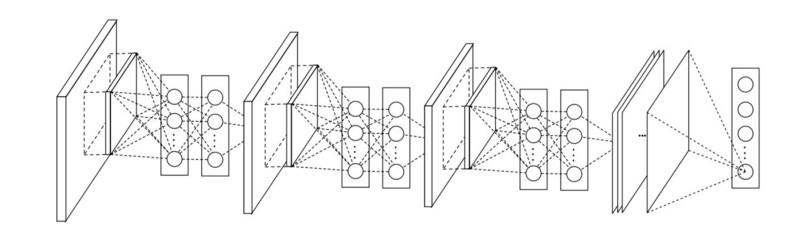
\includegraphics[scale = 0.5]{images/nin.jpg}
    \caption{Illustration NiN}
\end{figure}
\subsubsection{Inception module}
Inception module\cite{im1, im2, im3, im4} est une généralisation de NiN, dans chacune de ses couches on peut avoir plusieurs successions de couches convolutives de noyau de dimension (k$_i$,m$_i$) où les (k$_i$,m$_i$) ne sont pas nécessairement des couples de 1, les résultats de cet ensemble de couches successives sont fusionnés pour donner un ensemble d'images qui sont plus d'abstraction (profondeur). Un type de ce modèle a gagné le prix du challenge de la reconnaissance visuelle sur ImageNet en 2015 (GoogleNet \cite{im1}). Plusieurs amélioration de ce modèle ont été fait, il y a eu même une fusion avec le residual network qui donne plus de précision et permet de réduire le temps d'apprentissage également \cite{im1, im2, im3, im4}. Notre modèle s'inspire de ce type de réseau convolutif. 

\begin{figure}[H]
    \centering
    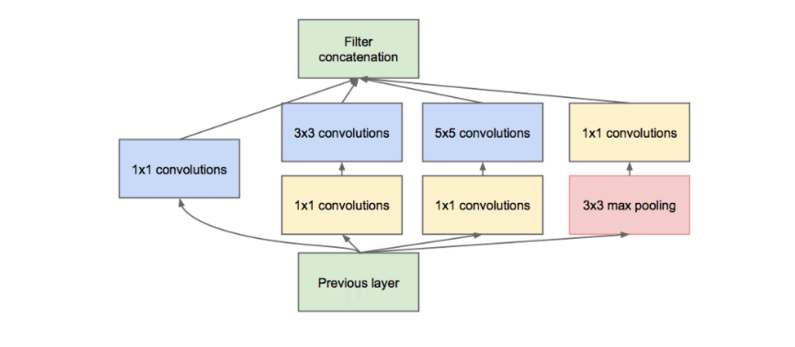
\includegraphics[scale = 0.5]{images/im.png}
    \caption{Illustration Inception module}
\end{figure}

%\subsubsection{Residual convolutional neural network}
\subsection{Couche d'agrégation (pooling)}
La couche d'agrégation permet non seulement la réduction de la dimension mais également permet de capturer certaines abstractions statistiques locales \cite{pool1, pool2, pool3, pool4}. Plusieurs couches d'agrégation ont été définies parmi elles la couche maxpooling et celle de averagePooling sont les plus utilisées. La couche maxpooling permet de choisir la valeur maximale locale parmi les valeurs de la région considérée et le averagepooling fait la moyenne de la région locale considérée.

\begin{figure}[H]
    \centering
    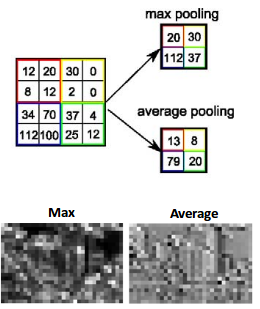
\includegraphics[scale = 0.5]{images/average_max.png}
    \caption{maxpooling et averagepooling}
\end{figure}


\section{Boosting}\label{section22}
Le boosting est une technique d'apprentissage qui s'appuie sur des modèles légers appris pour construire de modèles sophistiqués. Il opère de manière séquentielle d'un modèle à un autre tout en corrigeant l'erreur du précèdent en augmentant la distribution de ceux qui sont mal prédits. L'ensemble des modèles légers n'est pas nécessairement homogène, on peut faire le boosting avec plusieurs modèles de familles différentes. Ce type de modèle ne cessent de nous surprendre dans certains domaine par rapport aux réseaux de neurones profonds comme dans notre étude actuelle.

\textbf{Regularized gradient boosting tree}\\
Un arbre de décision est une fonction/modèle permet d'estimer une valeur ou classifier en construisant un arbre dont les feuilles sont les classes ou les valeurs estimées. Formellement un arbre de décision est décrit comme suit: \\ Soit $x \in R^n$ l'objet pour lequel une valeur y doit être prédite, $f$ la fonction correspondant à l'arbre de décision.
$f(x) = W_{q(x)}$ où $W \in R^d$  est le vecteur correspondant aux valeurs prédites et $q: R^n -> \{1..d\}$.

gradient boosting tree est la version du boosting où le modèle léger est un arbre de décision et l'ensemble de ces modèles est obtenu en minimisant le gradient, du passage d'un modèle à un autre. Pour éviter le problème du sur apprentissage, les techniques de régularisation sont appliquées. Supposons que nous avons $k$ estimateurs (modèles légers appris), l'estimation d'une valeur correspondante à $x$ est $\widehat{y} = \sum \limits_{i=1}^k f_i $ 

Le problème d'optimisation se résume à minimiser l'expression suivante : \\
$L(\Phi) = \sum \limits_{i=1}^n l(y, \widehat{y}) + \sum \limits_{j=1}^k \Omega(f_j)$ où $l(y, \widehat{y})$ est la fonction de perte, $\Omega(f_j)$ permet de contrôler la complexité du modèle pour empêcher le sur-apprentissage et $\Phi$ est l'ensemble de paramètres. $\Omega(f_j) = \frac{1}{2} \lambda \sum \limits_{i=1}^m W_{i}^2 + \alpha\sum \limits_{j = 1}^m |W_j| + \gamma m$, où $\lambda$, $\alpha$ et $\gamma$ sont des hyper-paramètres. \\Son implantation est xbboost, pour plus de détails on peut se référer cite{boost}.

\section{Apprentissage profond}
Le problème d'apprentissage se résume à un problème d'optimisation, çà revient à adapter les paramètres du modèle pour une généralisation du monde concerné (population) à partir d'un échantillon des données. L'apprentissage profond est l'adaptions des paramètres d'un modèle construit à partir de la superposition de plusieurs couches de réseau de neurones. La Superposition des couches permet de capturer plus d'abstractions. Ces paramètres sont appelés les poids (weights) du réseau.
\subsection{Apprentissage par rétro-propagation}
La rétro-propagation permet de propager l'erreur en arrière sur toutes les couches pour ajuster les poids.
\subsubsection{Optimisation}
Trouver les poids adaptés se ramène à optimiser une certaine fonction. Cette fonction dépend du type d'architecture de réseaux de neurones. La prédiction d'un individu X par une architecture de n couches en mode feed foward ou une architecture où les signes sont propagés dans un seul sens de l'entrée à la sortie (comme MLP) est $\widehat{Y} = Y_n$ tel que $Y_1 = \sigma(W_1*X + b_1)$, $Y_2 = \sigma(W_2*Y_1 + b_2)$, $... Y_n = \sigma(W_{(n-1)}*X + b_{(n-1)})$ où $W_i$ sont les poids du réseaux, $b_i$ les biais et $\sigma$ la fonction d'activation \cite{relu, rnna, erc}. Pour l'obtention des poids adaptés d'une architecture feed forward, il revient à minimiser la fonction $\sum \limits_{i=1}^m L(Y^i, \widehat{Y}^i)$ où $Y^i$ est la vraie valeur correspondante à X, m est la taille de l'échantillon et $L$ est la fonction de perte ainsi dans notre cas $L(Y, \widehat{Y}^i) = (\frac{Y-\widehat{Y}}{Y+1})^2$. Pour la minimisation, la descente du gradient est utilisée, pour chaque étape du gradient les paramètres et biais sont mis en jours. $W^i = W^{i-1} - \alpha \frac{\delta L}{\delta W} W^{i-1}$ où $\alpha$ est le taux d'apprentissage .\\

Le problème majeur du gradient est la difficulté d'obtention du minimum global, la rapidité de convergence et son coup de calcul. Plusieurs améliorations du gradient ont été effectuées concernant ces problèmes (SGD \cite{sgd_}, AdaGrad \cite{adagrad}, Adam \cite{adam}, ...). Pour ce travail Adam et SGD ont été utilisés.


\subsubsection{Régularisation}
La régularisation permet de contrôler la complexité du modèle en pénalisant la fonction à optimiser d'une certaine valeur. Ce qui permet au modèle de généraliser mieux le monde concerné et éviter le sur apprentissage. Plusieurs méthodes de régularisations existent:
\textbf{Batch normalisation \cite{batch}} qui normalise les données à l'entrée de la couche suivant la couche du batch, \textbf{L1 et L2} qui augmente sur la fonction de paramètres à optimiser la quantité respectivement $\lambda * \sum \limits_{i = 1}^m |w_i|$ et  $\lambda * \sqrt[\,] {\sum \limits_{i = 1}^m w_i^2} $)
 où $\lambda$ est un hyper-paramètre, et dropout qui supprime certains neurones d'une certaine proportionnalité $\alpha$ de la couche concernée. Dans ce travail batch normalisation, L2 et dropout ont été utilisés.
